\chapter[Proposta]{Proposta}
O objetivo deste capítulo é apresentar uma possível proposta de uma solução que atenda às necessidades colocadas no primeiro capítulo referente a problemática deste trabalho. A proposta está dividida em duas partes. A primeira parte está relacionada à coleta das métricas utilizando a ferramenta SonarQube, e a segunda parte está relacionada na criação do \textit{dashboard} e a visualização das informações. Para analise deste projeto foram escolhidos dois projetos, sendo o projeto PROJETO 1 e o PROJETO 2 de código aberto extraidos do portal do software publico brasileiro. A terceira e última parte do tarabalho consiste em analisar o trabalho realizado através de uma avaliação qualitativa de possíveis usuários.
\section{Coleta das Métricas}
Para fazer a coleta das métricas vai ser utilizado a ferramenta SonarQube que como já dito na seção de Suporte Tecnológico é muito utilizado em órgãos públicos e em editais por ser uma ferramenta \textit{open-source}. A coleta das métricas é feita de maneira dinamica em que o usuario decide qual suite de metricas vai utilizar, podendo utilizar uma customizada ou utilizar uma como base (neste projeto sera utilizada a do edital do DNPM \cite{edital}). As suites utilizadas neste trabalho são Suíte de Métricas de Chidamber-Kemerer e a Suíte MOOD.
O \textit{dashboard} será customizável de acordo com a necessidade do órgão. O ógão poderá escolher quais métricas deseja usar e qual a faixa de valores aceitáveis para as métricas, caso ele queira, também é possível utilizar uma suíte de métricas já customizada e com valores definidos. 
\\As métricas "Violações do tipo Blocker", "Violações do tipo Major" e "Violações do tipo Minor" são estipuladas de acordo com o próprio perfil do Sonar, chamado Sonar Way. Contudo a melhor maneira seria criar um perfil com as regras da própria organização garantindo uma avaliação mais focada no objetivo do orgão.
\\O objetivo deste trabalho é criar uma ferramenta que auxilie na auditoria de software entregue por empresas tercerizadas, contudo percebe-se que ainda que o trabalho possua grande aprovação ele nunca substituira o fator humano da auditoria, o software serve apenas como uma ferramenta de avaliação geral do software entregue. Recomenda-se que uma vez que o software seja submetido à ferramenta e seja aceito é necessário que seja feita uma auditoria em cima de uma amostragem do software entregue sob o olhar de um analista especializado para tal atividade.
\section{Criação do \textit{Dashboard}}
Com as informações obtidas o dashboard funcionará como uma tela para visualização dessas métricas. A solução é composta por duas telas, uma mostrando uma visão geral do projetos, e com indicadores quanto aprovação ou reprovação de cada projeto seguindo os limites estabelecidos pelo edital \cite{edital} que é de onde está sendo baseado as métricas e limites dos indicadores. A segunda tela consiste em uma visão mais detalhada sobre cada projeto mostrando a evolução do projeto em cada métrica e com um \textit{link} para o Sonar de cada métrica para um aprofundamento.

\section{Avaliação}
A avaliação do \textit{dashboard} será feita por parte de um gestor de tecnologia de um orgão público. Ele avaliará aspectos de usabilidade da ferramenta e se a ferramenta possuiria condições mínimas de ser implantada. Caso não seja possível essa avaliação com um profissional da área a avaliação será feita através de professores que possuem tal experiência com contratação de software para orgãos públicos também avaliando aspectos como usabilidade e melhorias necessárias para implantação em um orgão.
Para fazer está avaliação o gestor responderá a um questionário contendo 5 perguntas referentes ao uso e funcionalidades do software produzido. O questionário é igual ao da imagem \ref{img:questionario}

\graphicspath{{figuras/}}
\begin{figure}[h]
\centering
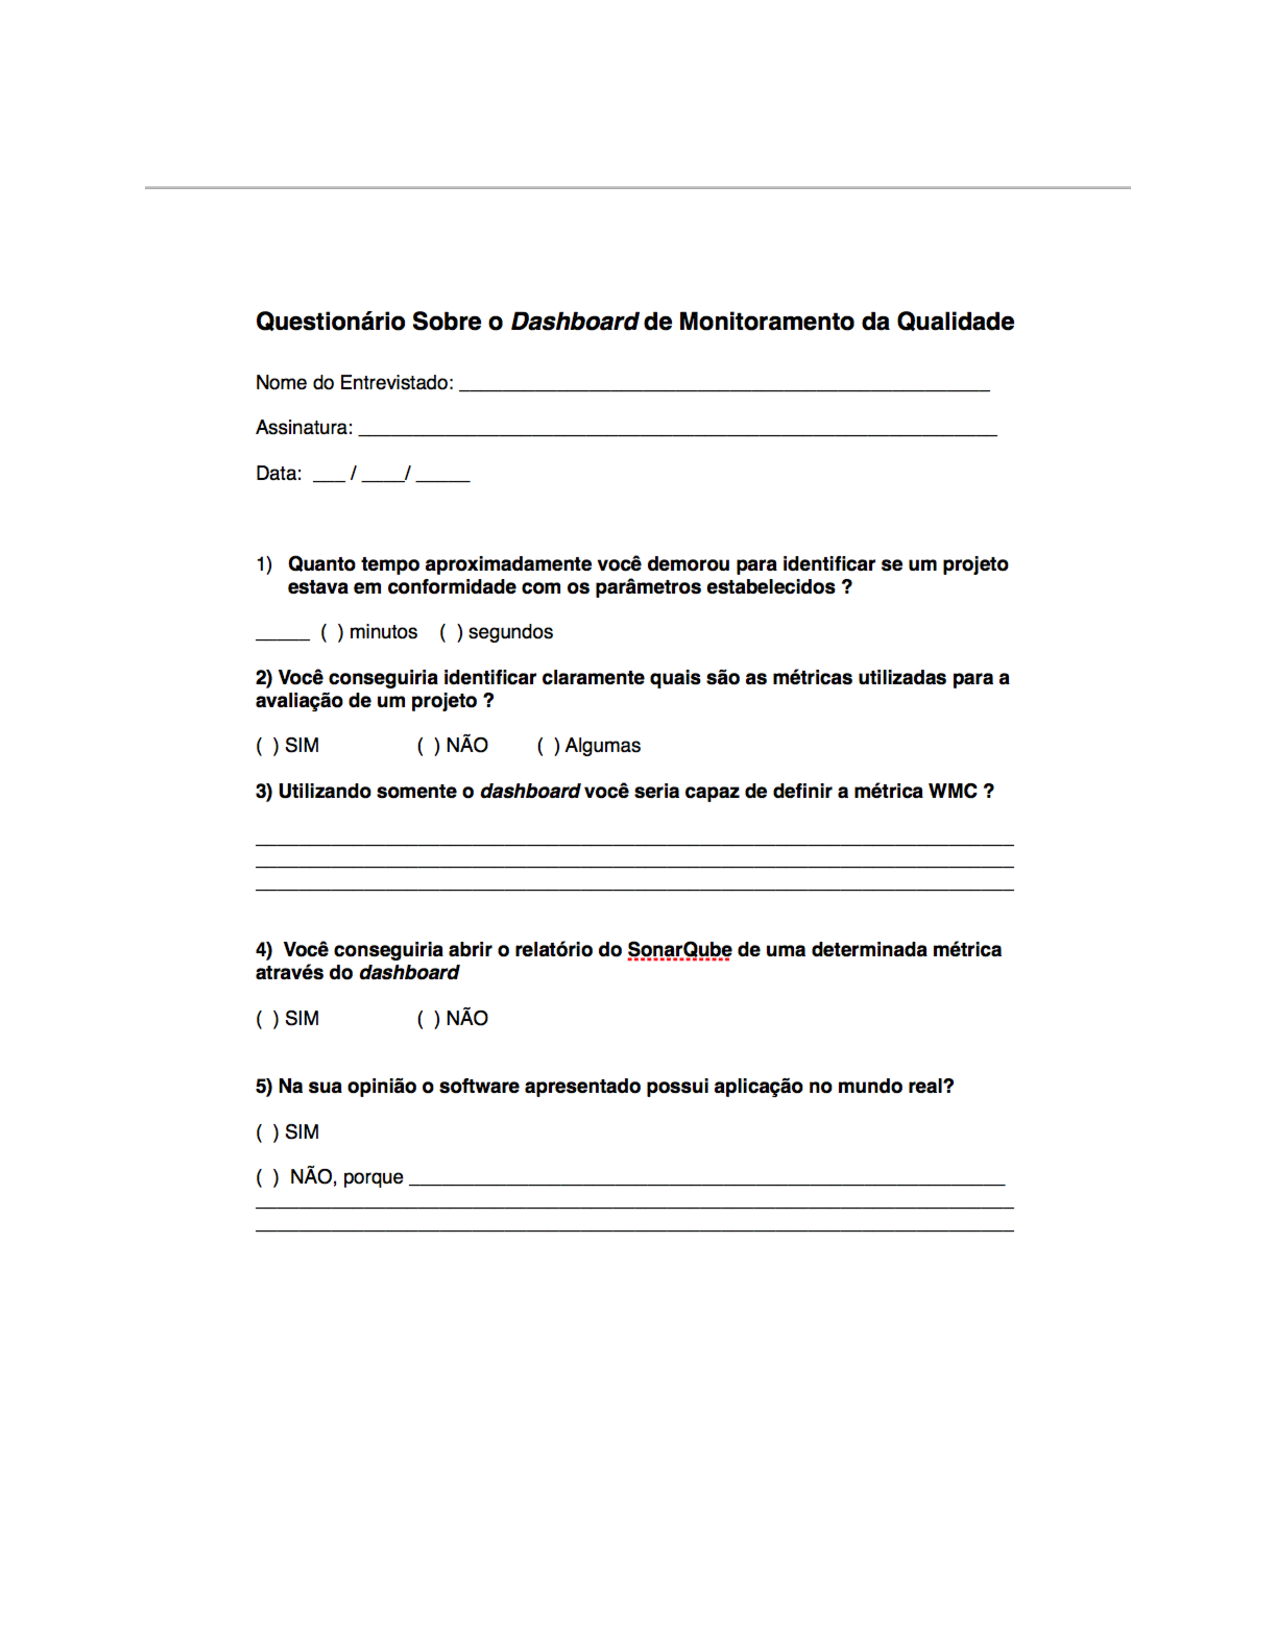
\includegraphics[scale=1.00]{questionario}
\caption{Questionário a ser aplicado ao fim do período de teste}
\label{img:questionario}
\end{figure}

\section{Resumo do Capítulo}
A proposta deste trabalho é criar uma maneira unificada de acompanhar a qualidade de código estático dos softwares entregues pela tercerizadas. Para fazer está analise a solução utiliza da ferramenta de analise estática SonarQube e de um conjunto de métricas relacionadas às boas práticas da programação. A solução encontrada é a utilização de um dashboard que mostre o real estado de um projeto e que através de indicadores seja possível determinar a saúde do código. A última etapa deste trabalho consiste na avaliação do trabalho produzido que será feito juntamente com um gestor de projeto de um órgão público ou um professor da insituição de ensino que responderá a um questionário quanto ao software produzido.